\section{PACT}\label{sec:PACT}
This Section is unless anything else is stated based upon \cite{Benyon}.

When designing an interactive system it is important to be human-centered, since it is the users who at the end determines the use of a given system.
\\\indent
Depending on how well designers have implemented a way to convey their conception of a given system, different users will interpret it differently.
Their interpretation, being based on individual understanding and knowledge, regulates the users interactions with the system and thereby determines what it really does, see \cref{fig:PACT-SystemImage}.

\begin{figure}[H]
	\centering
	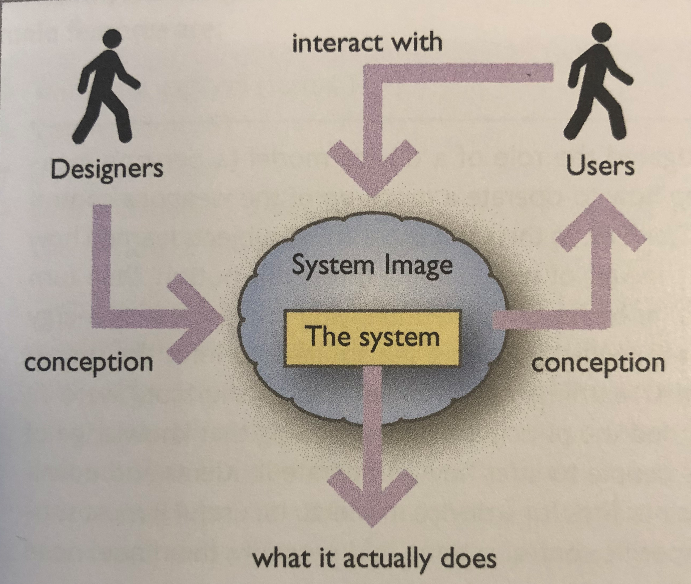
\includegraphics[width=0.4\textwidth]{billeder/SystemImage-Benyon.png}
	\caption{\textit{The System Image from
			\citep[p.~31]{Benyon} %Kan evt også bare skrive \cite{Benyon}
		}}
	\label{fig:PACT-SystemImage}
\end{figure}

To help understand and reflect upon the users and their relation to a interactive system, the framework PACT is used.
PACT is an acronym for ''people, activities, contexts and technologies'', see \cref{sec:PACT-method} for further details.
This analysis framework is used to analyze the users, such that developers are able to design the system people-centered instead of machine-centered.
%The method also helps developers to reflect upon how to best convey their conception and the essence of the system to the users and thereby influence users interactions with the system.

\subsection{The acronym outlined}\label{sec:PACT-method}
\subsubsection{People}
People differs from each others in many ways.
This element in the PACT analysis is a way to ponder upon these differences as well as a way to categorize the different users of a system.
Three differences usually discussed in this part of the analysis is:
\begin{itemize}
	\item Physiological
	\item Psychological
	\item Social
\end{itemize}

\textbf{Physiological differences} covers the relevant ways people differs in physical characteristics.
This could be, differences in perception from the five senses; sight, hearing, touch, smell and taste as well along with age, height or weight.
\begin{example}
As an example, when making an interface it is important to consider color blindness, since it affects about $8\%$ men and $0.5\%$ women in the world \cite{ColourBlind}.
\end{example}

\textbf{Psychological differences} describes things such as; emotional make-up, how stress affects different people, attention, memory and spatial ability.
Furthermore, is language and culture also important points to consider since these affect the psyche and thereby the way people interpret things.
\begin{example}
	In USA is a tick used when marking acceptance and a cross to mark rejection, while it in Britain can be used for both. Brits do among other use a cross on the voting paper.
\end{example}


\textbf{Social differences} is about how people use system for different reasons and therefore can have various goals.
Additionally, there is also a big difference in people expertise levels which affects how an interface might be designed.
\\\indent
This is an important consideration since designing a system for a homogeneous group of people is  distinct from designing one for a heterogeneous group.

\subsubsection{Activities}
First and foremost, when considering the activities the developers or designers should focus on the overall purpose of these. When that has been done one can begin considering the main features such as those described below:

\textbf{Temporal aspects} covers different features in the system as well as a consideration of how the users interaction with the system is done during a day.
\\\indent
Starting with the considerations of users interactions, one need to consider among other: How often is the interactive system used? And is the interactions with this system done continuously or interrupted?
\\\indent
For the temporal aspects in a given system the developers need to consider things such as; time preassures, peaks and troughs, and the response time of a given activity.


\textbf{Cooperation} is simply the consideration of whether or not the activity is done in cooperation with others or alone, and if a mix here of, then how and when the cooperation is needed.
\\\indent
This is an important consideration since a system which is i done in cooperation with others needs to have an awareness of others, be able to coordinate it between them and maybe have a communication system as well.
On the other hand if the activities is done completely alone these features are not necessary.

\textbf{Complexity} describe the question of how well-defined is the activity?
Is it a well-defined task which can be done in a simple step-by-step design?
Or is it a vague task, which would need users to browse around?

\textbf{Safety Critical} has two sides to it.
First is whether or not the activity in itself is ''safety-critical'' where mistakes could be reason for injury or serious accidents.
Second is the consideration of ''what will happen when mistakes and errors are made?'' which is an important for any developer to reflect upon and then design for these circumstances

\textbf{The nature of the content} is a more technical reflection of which data requirements are needed for the activity as well as what media it requires.

\subsubsection{Contexts}
Context also have more facets to it.
It can be thought of, as something that surrounds activities as well as a feature which binds them together into a whole.
Usually when considering this point in PACT the three points: Physical environment, Social context and Organizational context are at the main focus.
\\\indent
The physical environment might cover everything from weather to geographical placement of where the activity is done.
It is an analysis of the surrounding environment which may have effect on how users perform activities.
While Social context covers things such as whether or not the environment is supportive, or the user is alone in using and learning the activities.
It is also an reflection on if the social norms may dictate certain designs.
Lastly the organizational context is among other an examination of the impact new technology may have on the organization.
It is also a review of the circumstances under which the activities is done; time, place and so on.

\subsubsection{Technologies}
Technologies is the reflection on the medium which interactive system designers work with.
It covers looking into elements such as what medias and technologies is needed to best get input and present the output, and review the communication between the needed devices.
Furthermore, it also examines the content, which concerns the data in the system and its form.
Good content is defined as accurate, up to date, relevant and well presented.

\subsection{PACT analysis}\label{sec:PACT-analysis}
Based on the interviews with Pia,
% conslutant and acting quality chief at JBJ,
{\color{red} section XX}, the PACT analysis for the project described in this report is as follows.

\subsubsection*{People}

There are four main groups of people; the quality manager, the secretary, department heads and everyday workers.
This is a heterogeneous group with different levels of IT experience ranging from no skills with IT and therefore cautious about it, to the level of everyday office work.
The group also has different levels of domain expertise ranging from no to expert which needs to be considered. The quality manager is a domain expert and therefore has different needs of the system than the everyday worker with no expertise.
\newline
Furthermore, issues such as colorblindness, other eye handicap as well as bad memory need to be considered when designing the system and interface.

\subsubsection*{Activities}
The overall activities is to manage, update and access a handbook mostly the newest version but also possibly older versions as well.
It is needed to uphold standards set by the government to retain the companies certifications.
This is a well defined activity which takes place at least yearly, though sometimes more often.
\\\indent
When doing the activities users may experience interruptions and should therefore be simple to use and easy to get back to.
The activities would most often be done during business hours, from 8-16 on weekdays,though may be accessed outside of this time frame as well.
Additionally, the activities is mostly done alone but may be done in collaboration with others, though this is not required.
\\\indent
The data to be entered into the system are mostly larger data entries and possibly many of such.
\\\indent
The activities is in themselves not safety-critical but integrity is a very important aspect since mistakes can cause money-loss or loss of certification.

\subsubsection*{Contexts}
\todo[inline]{Mangler}




\subsubsection*{Technologies}
Since the activities are most often be done in a office environment on a standard PC the input medias are Keyboard and mouse.
In addition output is presented through a visual screen picture, or for the workers on the factory floor a printed version of the handbook, or parts of it.
\\\indent
The contents are presented through a General User Interface (GUI).
Furthermore, the communication user-to-user is usually done through telephone, while it between devices are done over a Network, such as Wi-fi.
Lastly, is the communication from the system to a user which is done through notifications.

% I like this - Rasmus
